\documentclass[12pt,a4paper]{ctexart}
\usepackage[left=2.5cm,right=2.5cm,top=2.6cm,bottom=2.5cm]{geometry}
\usepackage{amsmath,amssymb,bm,mathtools}
\usepackage{booktabs,tabularx,array,multirow,threeparttable}
\usepackage{graphicx,float,caption,subcaption}
\usepackage{tikz}
\usetikzlibrary{arrows.meta,positioning,shapes.geometric}
\usepackage{enumitem}
\usepackage{xcolor}
\usepackage{listings}
\usepackage{fancyhdr}
\usepackage{titlesec}
\usepackage{hyperref}

\hypersetup{colorlinks=true,linkcolor=black,citecolor=black,urlcolor=blue}
\captionsetup{font=small,labelsep=quad}
\setlength{\parindent}{2em}
\setlength{\parskip}{0pt}
\setlength{\emergencystretch}{2em}
\renewcommand{\baselinestretch}{1.25}
\newcolumntype{Y}{>{\centering\arraybackslash}X}
\pagestyle{fancy}
\fancyhf{}
\cfoot{\thepage}
\renewcommand{\headrulewidth}{0pt}
\titleformat{\section}{\centering\heiti\zihao{3}}{\chinese{section}、}{0.5em}{}
\titleformat{\subsection}{\heiti\zihao{4}}{\arabic{section}.\arabic{subsection}}{0.5em}{}
\lstset{
  language=Matlab,basicstyle=\footnotesize\ttfamily,
  numbers=left,numberstyle=\scriptsize\color{gray},
  frame=single,breaklines=true,showstringspaces=false,
  keywordstyle=\color{blue!70!black},commentstyle=\color{green!40!black},
  backgroundcolor=\color{gray!6},tabsize=4
}

\begin{document}

\begin{center}
{\heiti\zihao{2}基于时空几何遮蔽与分层优化的烟幕干扰弹投放策略}
\end{center}

\vspace{0.6em}
\noindent\textbf{摘\quad 要：}
针对无人机投放烟幕干扰弹阻断来袭导弹视线的问题，本文建立了包含导弹、无人机、烟幕弹及烟幕云团的统一时空运动模型，并以圆柱形真目标的可见表面为对象构造严格几何遮蔽判据。首先，根据导弹与无人机的匀速直线运动、烟幕弹的抛体运动以及云团的匀速下沉规律，给出投放点、起爆点和云团中心位置的解析表达式；随后利用点到视线段距离判断单个目标点是否被烟幕遮挡，并以多云团覆盖并集刻画完整目标的联合遮蔽。在求解方面，采用连续接近度指标引导差分进化进入有效区域，再以严格的离散几何模型进行局部修正和结果验收。对于多无人机、多导弹情形，进一步设计“候选任务分配--联合精修--冗余删除--增量投弹--分块再优化”的分层算法。

计算结果表明：问题1中烟幕弹投放点坐标为（17620，0，1800），起爆点坐标为（17188，0，1736.496），严格有效遮蔽时长为 $1.390$ s；问题2优化后时长为 $4.580$ s；问题3中三枚烟幕弹的联合遮蔽时长为 $6.410$ s；问题4中三架无人机联合遮蔽时长为 $11.170$ s。问题5最终保留9枚具有正边际贡献的烟幕弹，对 M1、M2、M3 的遮蔽时长分别为 $9.960$ s、$12.500$ s 和 $6.120$ s，总时长达到 $28.580$ s。高密度复算总时长仍为 $28.580$ s。进一步将20套整航线候选转化为0--1整数规划，分支定界最优性间隙为0，证明当前方案为候选集和给定离散精度下的全局最优组合。时间步长与目标采样收敛检验说明各问误差处于 $0.01\sim0.05$ s量级，方案具有较好的数值稳定性。

\noindent\textbf{关键词：}烟幕干扰；视线遮蔽；差分进化；分块优化；0--1整数规划

\section{问题重述}

某型无人机可在接到任务后瞬时调整航向，之后以 $70\sim140$ m/s 的速度等高度匀速直线飞行。无人机投放的烟幕干扰弹脱离载机后做抛体运动，起爆后瞬时形成半径为10 m的球形有效烟幕区域。云团中心以3 m/s的速度竖直下沉，起爆后20 s内可提供有效遮蔽。同一架无人机连续投放两枚烟幕弹的时间间隔不得小于1 s。

三枚来袭导弹均以300 m/s匀速飞向位于坐标原点的假目标，真目标为下底面圆心位于 $(0,200,0)$、半径7 m、高10 m的圆柱。需要针对五种情形确定无人机航向、速度、投放时刻和起爆延迟，使导弹观察真目标的视线被烟幕遮蔽的累计时间尽可能长。

五个问题由单弹给定策略计算逐步扩展为单机单弹优化、单机三弹优化、三机单弹协同以及五机多弹多目标协同。核心难点在于：遮蔽函数具有明显的0--1跳变；同一烟幕可能参与多个时段或多个目标点的联合遮蔽；问题5同时含有连续航迹变量、连续投弹变量和离散任务分配变量。

\section{问题分析}

\subsection{统一运动关系}

导弹、无人机、烟幕弹和烟幕云团均具有明确的运动规律。无人机航向和速度确定后，投放点可直接计算；烟幕弹在水平方向继承无人机速度，在竖直方向做自由落体；起爆后不再保留原水平速度，而形成定点生成并竖直下沉的烟幕云团。因此，各阶段位置均可表示为时间和决策变量的显式函数。

\subsection{遮蔽判定的几何本质}

导弹是否发现真目标，取决于导弹与真目标可见表面之间的视线是否穿过有效烟幕球。仅判断目标中心会忽略圆柱尺寸，故本文离散圆柱的可见侧面和顶面，对每个可见采样点分别计算烟幕中心到导弹--采样点线段的最短距离。当所有可见点均被至少一个烟幕球覆盖时，认定该时刻真目标被完整遮蔽。

\subsection{非光滑优化与分层求解}

严格遮蔽时间在大部分参数区域恒为零，直接使用智能算法容易陷入平台。本文以中心视线附近的连续 Logistic 接近度作为搜索代理，负责把候选带入有效区域；最终目标值始终由严格完整目标判据计算。对于问题5，先生成无人机--导弹候选任务，再进行组合选择和连续精修，随后删除冗余弹，并针对遮蔽空缺增量增加烟幕弹。最后用整数规划对有限候选库进行组合最优性认证。

\begin{figure}[H]
\centering
\begin{tikzpicture}[node distance=8mm and 9mm,>=Stealth,
box/.style={draw,rounded corners,align=center,minimum height=9mm,minimum width=28mm,fill=blue!5},
res/.style={draw,rounded corners,align=center,minimum height=9mm,minimum width=30mm,fill=green!8}]
\node[box] (kin) {运动学建模};
\node[box,right=of kin] (geo) {完整目标\\遮蔽判定};
\node[box,right=of geo] (proxy) {连续代理\\全局搜索};
\node[box,below=of proxy] (joint) {组合选择与\\分块精修};
\node[box,left=of joint] (add) {增量投弹与\\冗余删除};
\node[box,left=of add] (milp) {0--1整数规划\\候选集认证};
\node[res,below=of add] (verify) {高密度复算与\\收敛检验};
\draw[->] (kin)--(geo);\draw[->] (geo)--(proxy);\draw[->] (proxy)--(joint);
\draw[->] (joint)--(add);\draw[->] (add)--(milp);\draw[->] (milp)|-(verify);
\draw[->] (add)--(verify);
\end{tikzpicture}
\caption{总体建模与求解流程}
\end{figure}

\section{模型假设}

在不改变题目主要物理关系的前提下，作如下假设：

\begin{enumerate}[label=\arabic*)]
\item 导弹在研究时段内保持300 m/s匀速直线飞行，方向始终指向假目标原点；
\item 无人机接到任务后可瞬时改变航向，随后保持定高、定速、直线飞行，不计转向过渡过程；
\item 烟幕弹脱离无人机后水平方向速度不变，竖直方向仅受重力作用，取 $g=9.8$ m/s$^2$；
\item 烟幕弹起爆后瞬时形成球形有效区域，云团不考虑水平漂移，仅以3 m/s匀速下沉；
\item 云团有效半径为10 m，有效期为起爆后20 s；为避免贴地起爆的浮点误判，数值计算要求起爆高度不低于1 m，但最终方案最低高度远高于该阈值；
\item 不考虑无人机、导弹和烟幕弹之间的碰撞，也不考虑风场、空气阻力和烟幕扩散形变；
\item 不同烟幕弹的有效区域可以重叠，完整遮蔽由所有有效云团的覆盖并集共同决定。
\end{enumerate}

\section{符号说明}

\begin{table}[H]
\centering
\caption{主要符号及含义}
\begin{tabularx}{0.94\textwidth}{cXc}
\toprule
符号 & 含义 & 单位\\
\midrule
$\bm m_j^0$ & 导弹 $M_j$ 的初始位置 & m\\
$\bm u_k^0$ & 无人机 FY$k$ 的初始位置 & m\\
$v_M$ & 导弹速度，取300 & m/s\\
$v_k,\theta_k$ & 无人机 FY$k$ 的速度和航向角 & m/s，$^\circ$\\
$t_{ki}^{d}$ & 第 $i$ 枚烟幕弹的投放时刻 & s\\
$\tau_{ki}$ & 投放至起爆的延迟 & s\\
$t_{ki}^{b}$ & 起爆时刻，$t_{ki}^{b}=t_{ki}^{d}+\tau_{ki}$ & s\\
$\bm d_{ki},\bm b_{ki}$ & 投放点与起爆点 & m\\
$\bm c_{ki}(t)$ & 起爆后烟幕云团中心位置 & m\\
$R_s$ & 烟幕有效半径，取10 & m\\
$H_j(t)$ & 导弹 $M_j$ 在时刻 $t$ 的完整遮蔽指标 & --\\
$T_j$ & 对导弹 $M_j$ 的累计有效遮蔽时间 & s\\
\bottomrule
\end{tabularx}
\end{table}

\section{运动学与遮蔽判定模型}

\subsection{导弹运动模型}

设假目标为原点，导弹 $M_j$ 初始位置为 $\bm m_j^0$。其单位飞行方向为
\begin{equation}
\bm e_j^M=-\frac{\bm m_j^0}{\|\bm m_j^0\|_2}.
\end{equation}
因此导弹位置为
\begin{equation}
\bm m_j(t)=\bm m_j^0+v_Mt\bm e_j^M,\qquad
0\le t\le T_j^M=\frac{\|\bm m_j^0\|_2}{v_M}.
\end{equation}
三枚导弹到达假目标的时间约为66.999 s、63.750 s和60.367 s。

\subsection{无人机与烟幕弹运动模型}

无人机 FY$k$ 航向角为 $\theta_k$，速度为 $v_k$，水平单位方向为
\begin{equation}
\bm e_k^U=(\cos\theta_k,\sin\theta_k,0).
\end{equation}
无人机位置为
\begin{equation}
\bm u_k(t)=\bm u_k^0+v_kt\bm e_k^U.
\end{equation}
第 $i$ 枚烟幕弹在 $t_{ki}^{d}$ 投放，其投放点为
\begin{equation}
\bm d_{ki}=\bm u_k^0+v_kt_{ki}^{d}\bm e_k^U.
\end{equation}
起爆时刻为 $t_{ki}^{b}=t_{ki}^{d}+\tau_{ki}$，起爆点为
\begin{equation}
\bm b_{ki}=\bm u_k^0+v_kt_{ki}^{b}\bm e_k^U
-\left(0,0,\frac{1}{2}g\tau_{ki}^2\right).
\end{equation}
起爆后云团中心为
\begin{equation}
\bm c_{ki}(t)=\bm b_{ki}-(0,0,3(t-t_{ki}^{b})),\quad
t_{ki}^{b}\le t\le t_{ki}^{b}+20.
\end{equation}

\subsection{点到视线段距离}

设某时刻导弹位置为 $\bm m$，目标采样点为 $\bm q$，云团中心为 $\bm c$。导弹到目标点的视线段可写为
\begin{equation}
\bm \ell(\lambda)=\bm m+\lambda(\bm q-\bm m),\qquad 0\le\lambda\le1.
\end{equation}
投影系数为
\begin{equation}
\lambda^*=\operatorname{clip}_{[0,1]}
\frac{(\bm c-\bm m)^{\mathsf T}(\bm q-\bm m)}
{\|\bm q-\bm m\|_2^2}.
\end{equation}
云团中心到视线段的最短距离为
\begin{equation}
d(\bm c,\overline{\bm m\bm q})=
\left\|\bm c-\bm m-\lambda^*(\bm q-\bm m)\right\|_2.
\end{equation}
当 $d\le R_s$ 且云团处于有效期内时，该云团可以遮挡导弹对采样点 $\bm q$ 的视线。

\subsection{完整圆柱目标遮蔽}

将圆柱侧面按圆周角和高度离散，并在顶面设置若干同心圆采样点。根据导弹位置剔除不可见侧面点，得到时刻 $t$ 的可见点集合 $\mathcal Q_j(t)$。定义
\begin{equation}
h_{ijq}(t)=
\mathbf 1\left\{d\bigl(\bm c_i(t),\overline{\bm m_j(t)\bm q}\bigr)\le R_s\right\}.
\end{equation}
多云团联合遮蔽指标为
\begin{equation}
H_j(t)=\min_{\bm q\in\mathcal Q_j(t)}
\max_{i\in\mathcal A(t)}h_{ijq}(t),
\end{equation}
其中 $\mathcal A(t)$ 为时刻 $t$ 的有效云团集合。累计遮蔽时间为
\begin{equation}
T_j=\int_0^{T_j^M}H_j(t)\,\mathrm dt.
\end{equation}
数值计算采用离散时间网格和梯形积分，最终结果再用更小时间步长与更密集目标采样复算。

\subsection{连续搜索代理}

严格指标在绝大多数参数空间为零。为增强搜索方向性，定义连续接近度
\begin{equation}
S_j(t)=\max_i
\frac{1}{1+\exp[(d_{ij}(t)-R_s)/\sigma]},\qquad \sigma=2,
\end{equation}
并以 $\sum_j\int S_j(t)\,\mathrm dt$引导差分进化。代理指标只用于生成候选，正式结果始终由 $H_j(t)$评价。

\section{问题1：给定策略的遮蔽时长}

FY1以120 m/s沿 $x$ 轴负向飞行，故
\begin{equation}
\bm u_1(t)=(17800-120t,0,1800).
\end{equation}
在1.5 s投放，得到
\begin{equation}
\bm d_{11}=(17620,0,1800).
\end{equation}
延迟3.6 s起爆，起爆时刻为5.1 s，起爆点为
\begin{align}
x_b&=17620-120\times3.6=17188,\\
z_b&=1800-\frac12\times9.8\times3.6^2=1736.496.
\end{align}
所以
\begin{equation}
\bm b_{11}=(17188,0,1736.496).
\end{equation}
将导弹轨迹、云团下沉轨迹代入完整目标遮蔽模型，得到中心视线遮蔽时长1.436 s，完整圆柱目标严格遮蔽时长为
\begin{equation}
\boxed{T_1=1.390\ \mathrm{s}}.
\end{equation}

\section{问题2：单机单弹优化}

决策变量取为
\begin{equation}
\bm x=(\theta_1,v_1,t_d,\tau),
\end{equation}
满足
\begin{equation}
0\le\theta_1<360^\circ,\quad70\le v_1\le140,\quad
t_d\ge0,\quad\tau\ge0,\quad z_b\ge1.
\end{equation}
先用差分进化搜索连续代理目标，再用完整目标函数进行坐标局部修正。所得结果如表\ref{tab:p2}。

\begin{table}[H]
\centering
\caption{问题2最优投放参数}
\label{tab:p2}
\resizebox{\textwidth}{!}{
\begin{tabular}{cccccc}
\toprule
航向角/$^\circ$ & 速度/(m/s) & 投放时刻/s & 起爆延迟/s & 投放点 & 起爆点\\
\midrule
4.942 & 139.385 & 0.893 & 0 & $(17924,11,1800)$ & $(17924,11,1800)$\\
\bottomrule
\end{tabular}}
\end{table}

投放后立即起爆对应 $\tau=0$。题目未规定最小引信延迟，因此该边界解在本文模型中可行。严格遮蔽时长为
\begin{equation}
\boxed{T_1=4.580\ \mathrm{s}},
\end{equation}
较问题1提高约229.5\%。

\section{问题3：单机三弹时序优化}

同一无人机三枚弹共享航向和速度。采用参数化
\begin{equation}
t_1^d=x_3,\quad
t_2^d=x_3+1+x_4,\quad
t_3^d=x_3+2+x_4+x_5,
\end{equation}
从编码层面保证投弹间隔不小于1 s。为避免经验时间范围遗漏，分别搜索聚焦时间域、完整飞行时间域及三弹均衡候选，再按“总时长优先、近等价时有效弹数优先”的词典序规则选择。

\begin{table}[H]
\centering
\caption{问题3投放策略}
\begin{tabular}{cccccc}
\toprule
弹号 & 航向角/$^\circ$ & 速度/(m/s) & 投放时刻/s & 起爆延迟/s & 独立遮蔽/s\\
\midrule
1 & 5.414 & 140.000 & 0 & 0 & 2.560\\
2 & 5.414 & 140.000 & 1.000 & 0 & 4.110\\
3 & 5.414 & 140.000 & 5.731 & 4.877 & 0\\
\bottomrule
\end{tabular}
\end{table}

三枚弹联合严格遮蔽时长为
\begin{equation}
\boxed{T_1=6.410\ \mathrm{s}}.
\end{equation}
第三枚弹在当前总时长最优候选中未产生额外边际增益。另行搜索得到三弹均有效方案，但联合时长仅5.910 s，因此正式结果保留总时长较大的6.410 s方案。该结果说明“使用三枚弹”不等价于“三枚弹均增加联合时长”，论文不将其解释为三弹均有效。

\section{问题4：三机单弹协同优化}

三架无人机分别生成接近有效视线的单弹候选，再将12个连续变量联合局部修正。三枚烟幕弹的独立贡献及联合效果如图\ref{fig:p4bar}所示。

\begin{figure}[H]
\centering
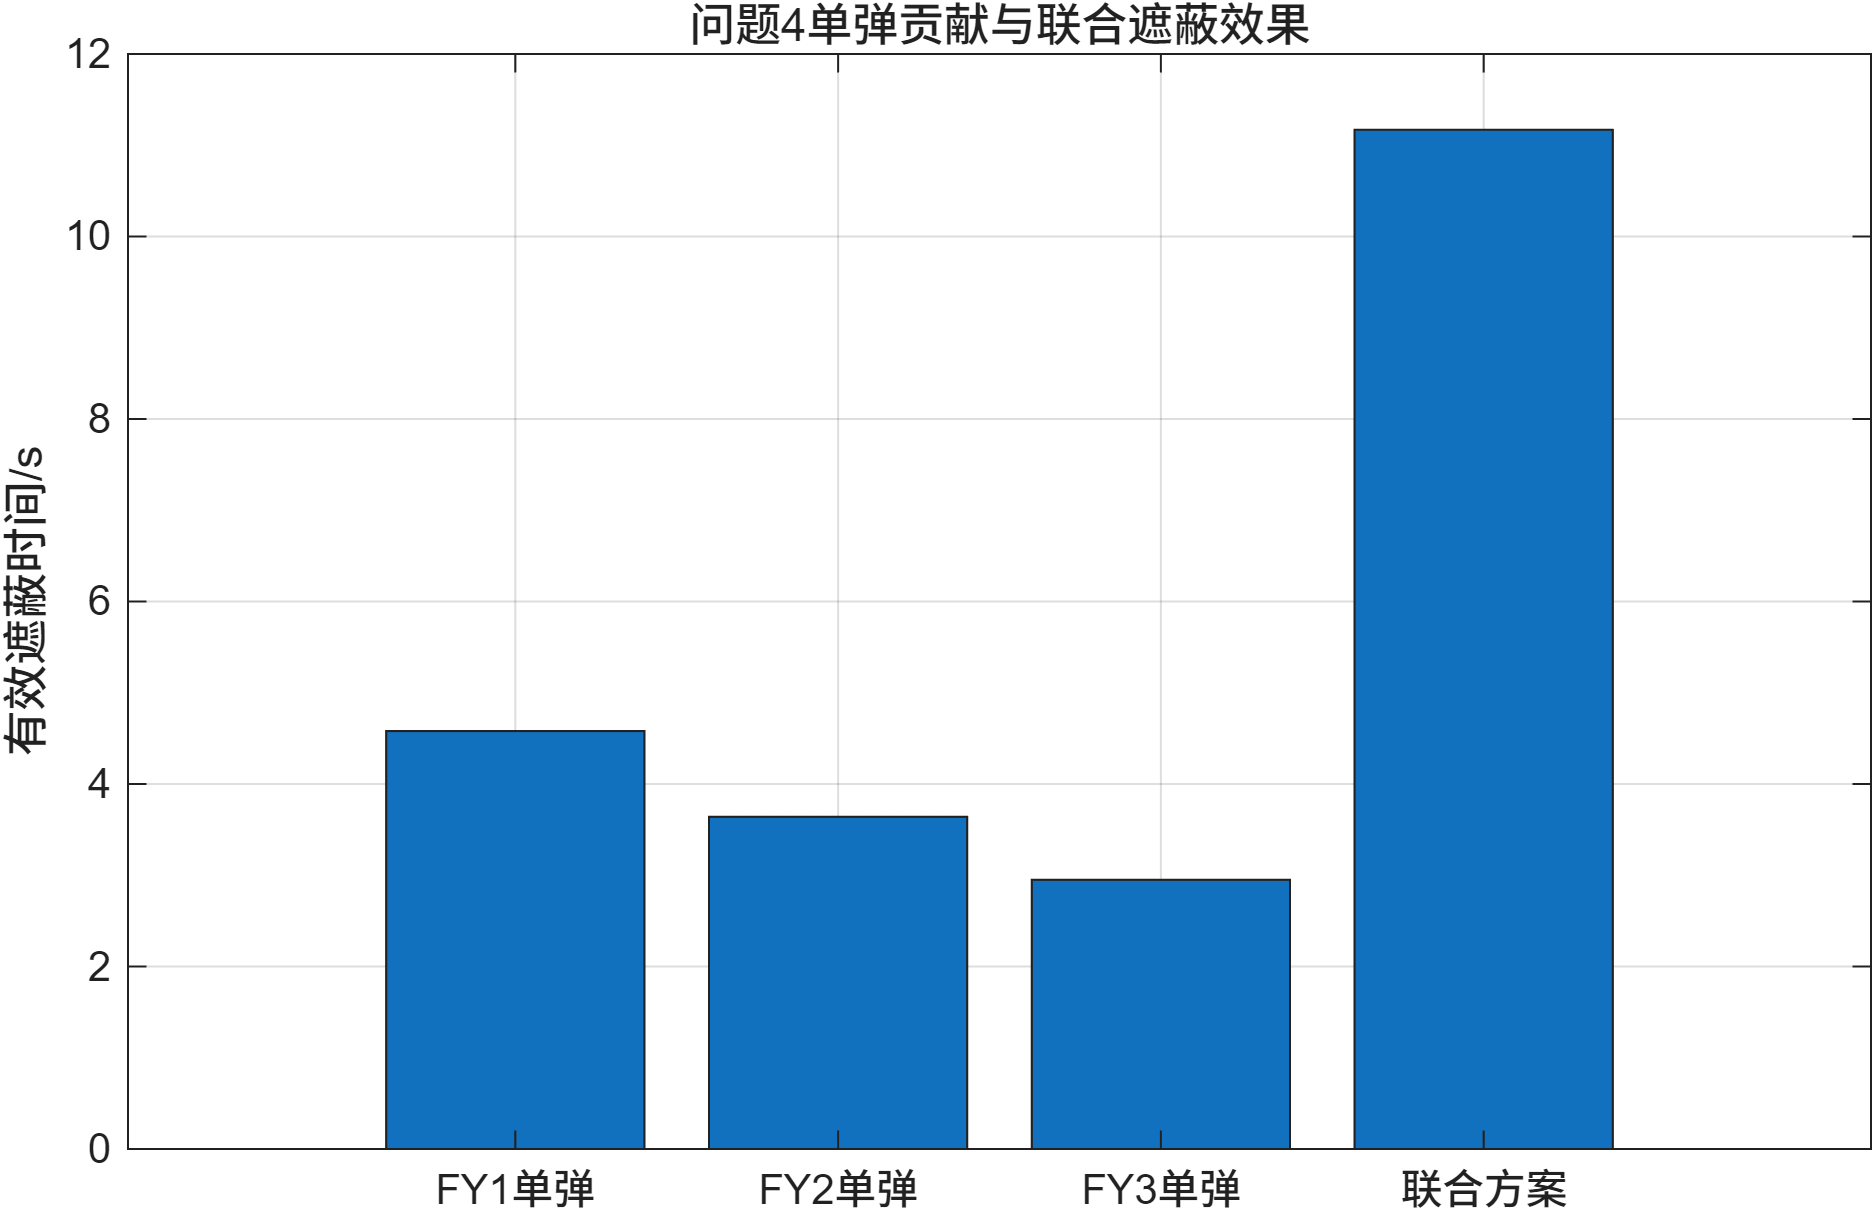
\includegraphics[width=0.72\textwidth]{figures/problem4_bar.png}
\caption{问题4单弹贡献与联合遮蔽效果}
\label{fig:p4bar}
\end{figure}

\begin{table}[H]
\centering
\caption{问题4三架无人机投放策略}
\begin{tabular}{cccccc}
\toprule
无人机 & 航向角/$^\circ$ & 速度/(m/s) & 投放/s & 延迟/s & 独立遮蔽/s\\
\midrule
FY1 & 4.942 & 139.385 & 0.893 & 0 & 4.580\\
FY2 & 238.700 & 103.265 & 7.929 & 7.416 & 3.640\\
FY3 & 89.251 & 115.591 & 22.629 & 4.087 & 2.950\\
\bottomrule
\end{tabular}
\end{table}

三弹独立时长之和为11.170 s，联合严格遮蔽时间同样为
\begin{equation}
\boxed{T_1=11.170\ \mathrm{s}}.
\end{equation}
高密度复算为11.150 s，差异仅0.020 s，三架无人机均具有正边际贡献。

\section{问题5：五机多弹多目标协同优化}

\subsection{分层优化框架}

问题5约含40个连续变量并伴随离散任务分配，直接联合搜索容易陷入大面积零值平台。本文采用以下步骤：

\begin{enumerate}[label=\arabic*)]
\item 针对每个“无人机--导弹”组合生成三弹候选航线；
\item 枚举五架无人机的任务分配组合，以完整圆柱目标遮蔽时间进行筛选；
\item 对选中组合按无人机分块调整航向、速度、投放时刻和起爆延迟；
\item 计算删除边际贡献，在总时长和最短目标时长容差内删除冗余弹；
\item 提取当前遮蔽空缺，搜索新增弹，并将新增弹与对应航线联合优化；
\item 循环执行“增加--精修--验收”，无增益时停止，再进行一次最终冗余删除；
\item 以高密度完整目标模型复算，并用0--1整数规划认证候选集组合最优性。
\end{enumerate}

正式接受规则为：若总时长提高超过0.01 s则接受；若总时长下降不超过0.02 s，则仅在最短目标时长提高超过0.01 s时接受。该规则保证总遮蔽时长始终为主目标。

\subsection{最终航迹和投放策略}

最终使用9枚烟幕弹。五架无人机航向与速度见表\ref{tab:p5route}，具体投放参数见表\ref{tab:p5bomb}。

\begin{table}[H]
\centering
\caption{问题5无人机航向与速度}
\label{tab:p5route}
\begin{tabular}{ccc}
\toprule
无人机 & 航向角/$^\circ$ & 速度/(m/s)\\
\midrule
FY1 & 5.608 & 139.897\\
FY2 & 295.947 & 96.503\\
FY3 & 95.932 & 96.570\\
FY4 & 259.905 & 140.000\\
FY5 & 117.096 & 137.947\\
\bottomrule
\end{tabular}
\end{table}

\begin{table}[H]
\centering
\caption{问题5烟幕弹投放与起爆参数}
\label{tab:p5bomb}
\resizebox{\textwidth}{!}{
\begin{tabular}{cccccccc}
\toprule
无人机 & 弹序 & 投放/s & 延迟/s & 投放点 $(x,y,z)$/m & 起爆点 $(x,y,z)$/m & 主要目标 & 独立时长/s\\
\midrule
FY1&1&0&0&(17800,0,1800)&(17800,0,1800)&M1&2.560\\
FY1&2&1.000&0&(17939,14,1800)&(17939,14,1800)&M1&4.040\\
FY2&1&10.000&1.188&(12422,532,1400)&(12472,429,1393)&M2&2.800\\
FY2&2&11.343&0.021&(12479,416,1400)&(12480,414,1400)&M2&3.680\\
FY3&1&25.690&4.272&(5744,-532,700)&(5701,-122,611)&M3&2.500\\
FY3&2&30.000&3.750&(5701,-118,700)&(5663,242,631)&M2&2.460\\
FY4&1&0.866&10.968&(10979,1881,1800)&(10710,369,1210)&M2&3.480\\
FY4&2&2.250&12.000&(10945,1690,1800)&(10650,36,1094)&M1&3.540\\
FY5&1&12.780&0.280&(12197,-431,1300)&(12179,-396,1300)&M3&3.620\\
\bottomrule
\end{tabular}}
\end{table}

\begin{figure}[H]
\centering
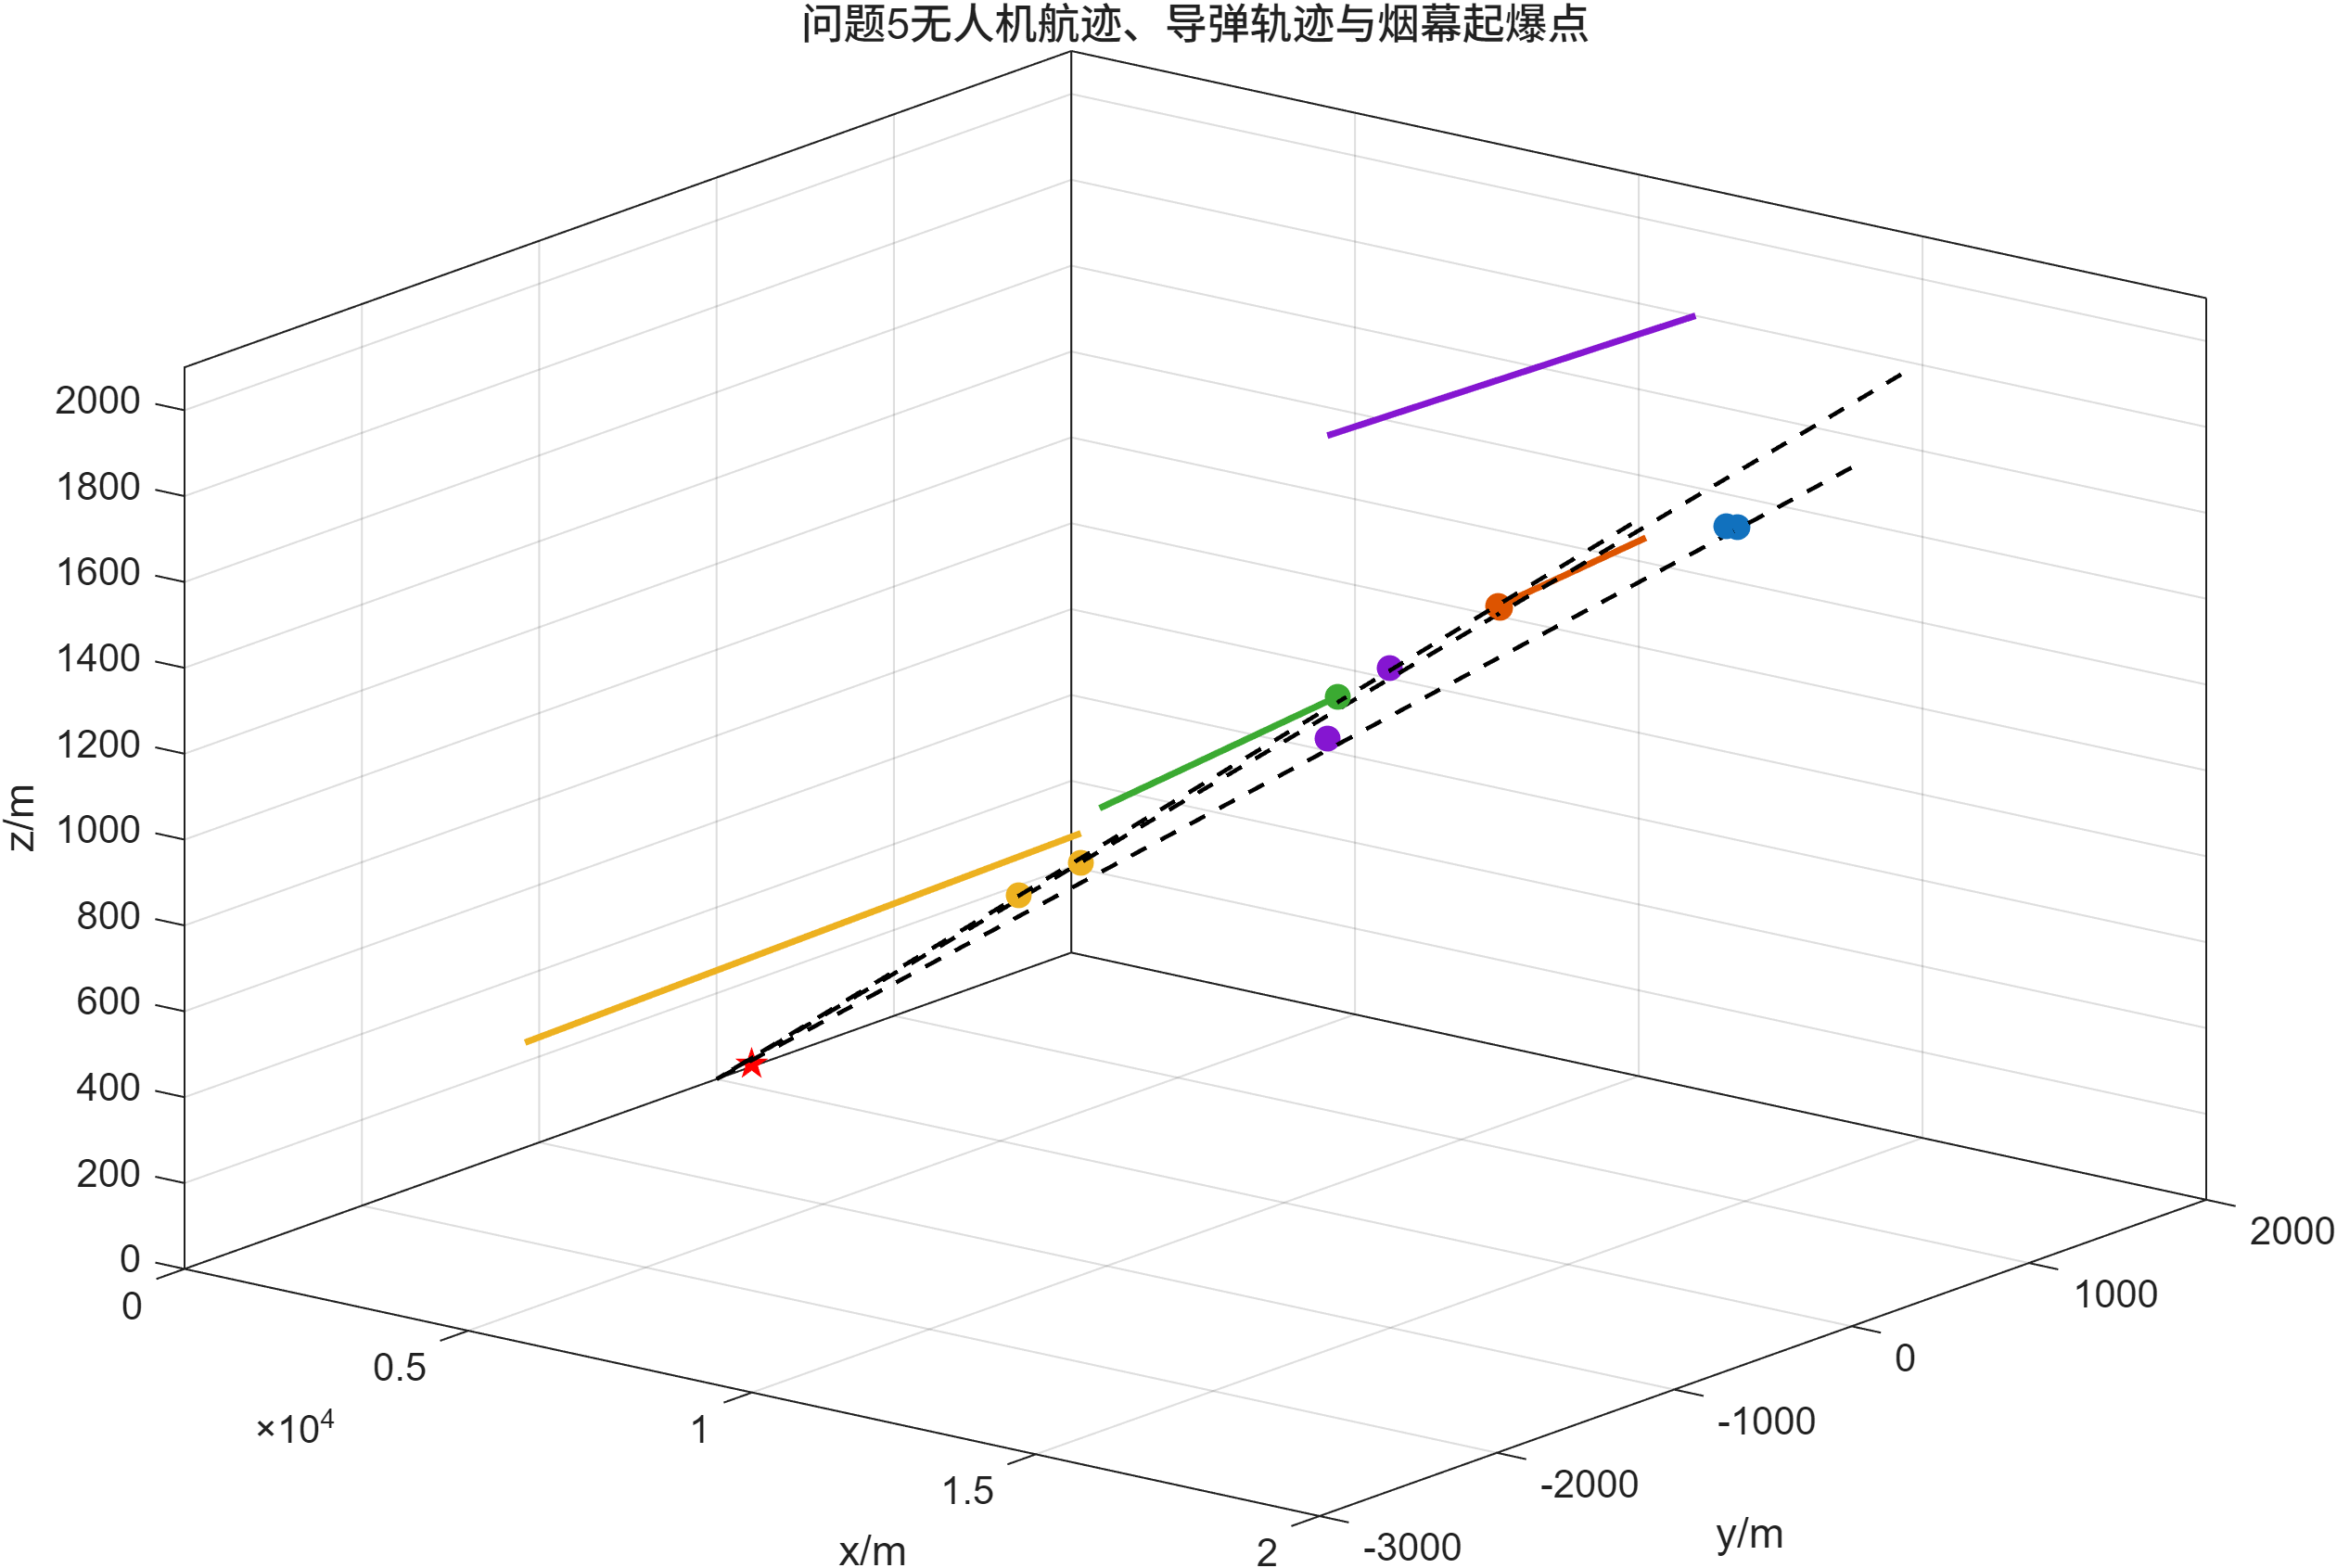
\includegraphics[width=0.88\textwidth]{figures/trajectory_p5.png}
\caption{问题5无人机航迹、导弹轨迹与烟幕起爆点}
\end{figure}

\subsection{遮蔽结果与区间分析}

三枚导弹的严格遮蔽结果为
\begin{equation}
(T_1,T_2,T_3)=(9.960,12.500,6.120)\ \mathrm{s},
\end{equation}
总时长为
\begin{equation}
\boxed{T_{\mathrm{sum}}=28.580\ \mathrm{s}}.
\end{equation}

\begin{figure}[H]
\centering
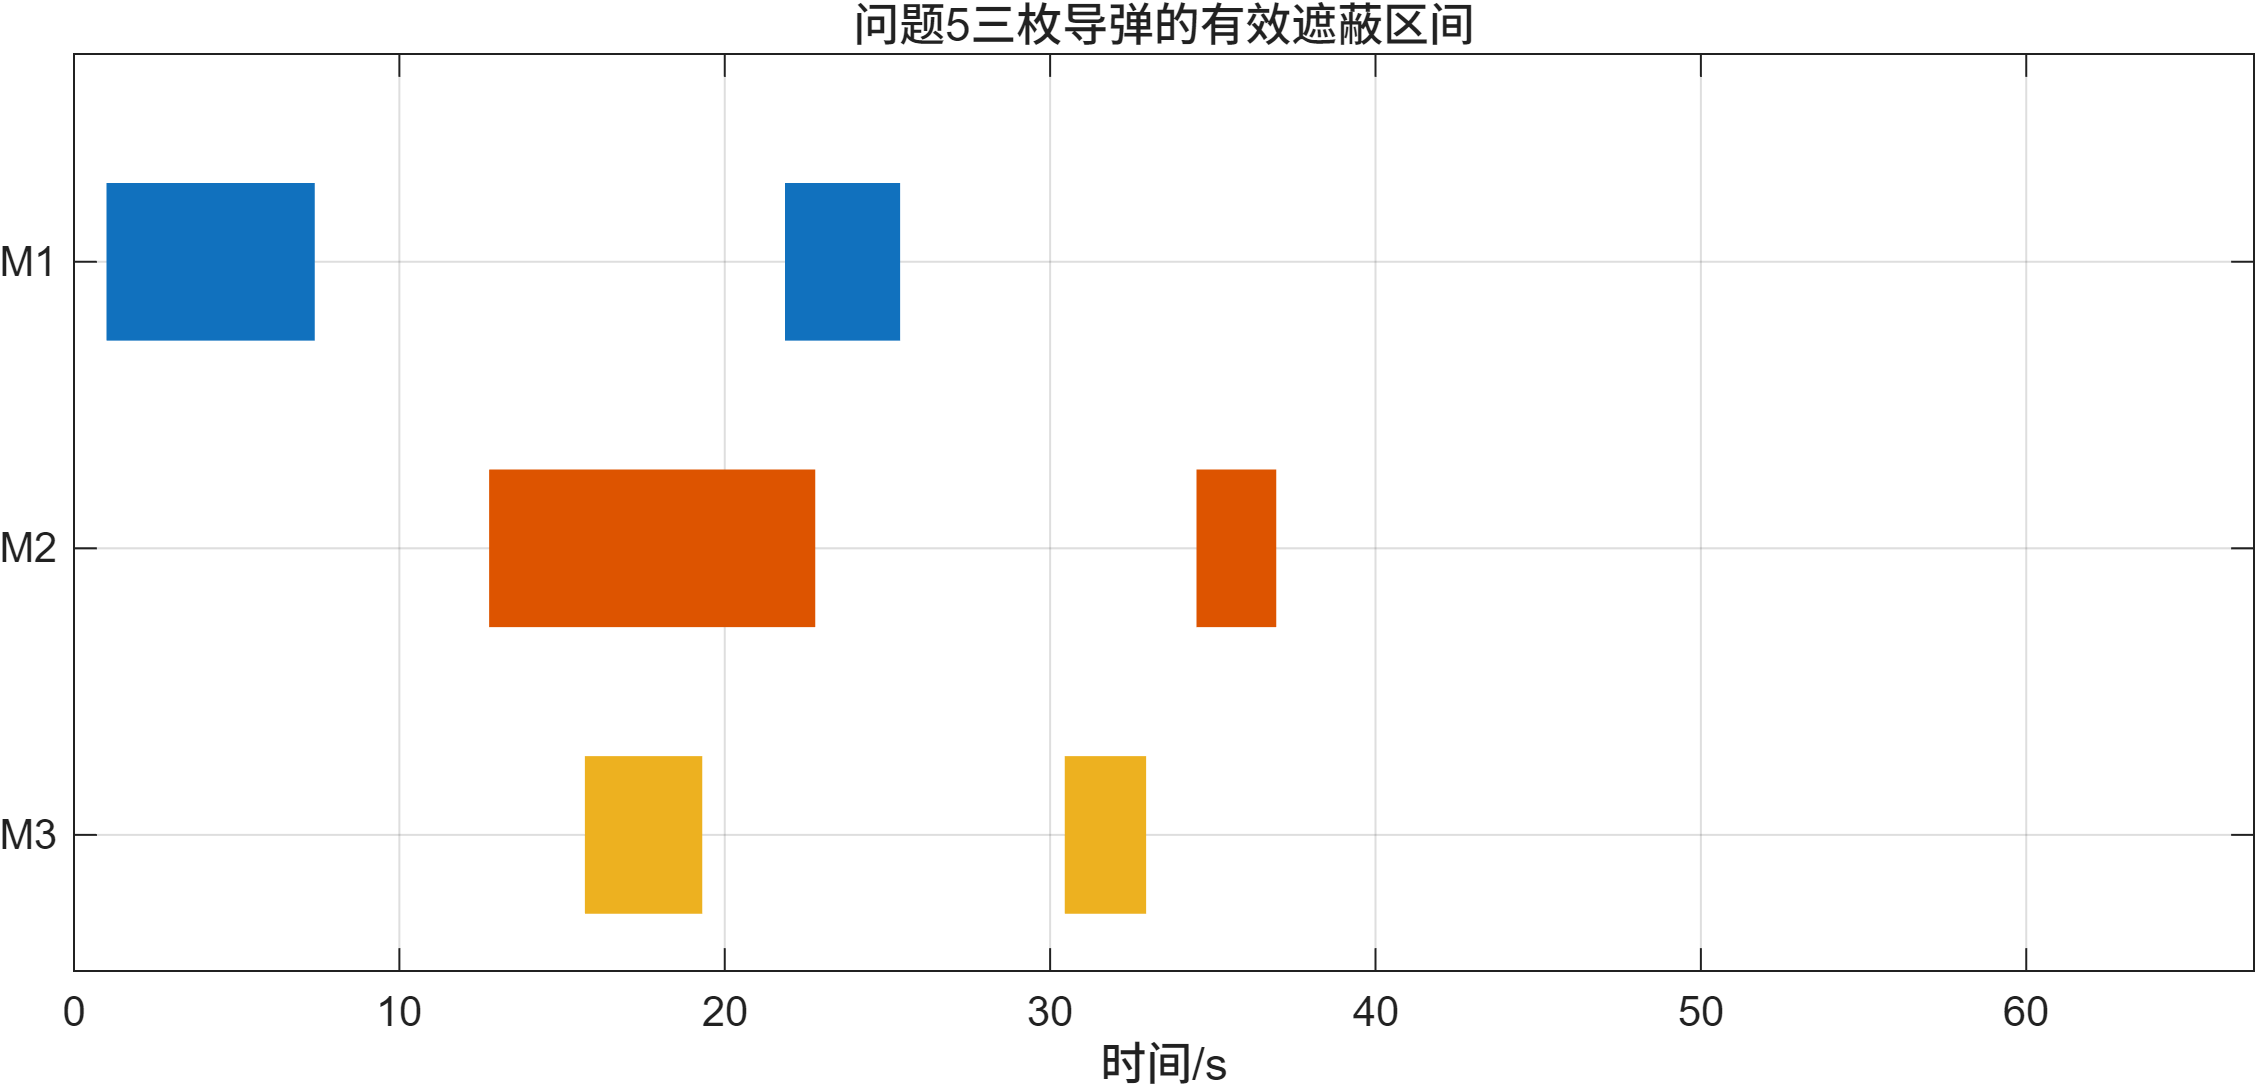
\includegraphics[width=0.86\textwidth]{figures/intervals_p5.png}
\caption{问题5三枚导弹的有效遮蔽区间}
\end{figure}

M1在约 $1.00\sim7.40$ s和 $21.85\sim25.39$ s受到遮蔽；M2在约 $12.76\sim22.78$ s和 $34.50\sim36.95$ s受到遮蔽；M3在约 $15.70\sim19.31$ s和 $30.45\sim32.95$ s受到遮蔽。各区间允许不连续，符合题意。M2遮蔽时间较长是总时长优先目标下的自然结果；若任务更强调均衡，可在总时长容差内进一步最大化 $\min(T_1,T_2,T_3)$。

\subsection{候选集整数规划认证}

每架无人机保留当前正式航线及分别针对三枚导弹形成的三套候选，共20套整航线方案。设 $x_p$表示是否选择方案 $p$，$y_{jn}$表示导弹 $j$ 在离散时刻 $t_n$是否完整遮蔽，预计算点级遮蔽矩阵 $a_{pjnq}$，建立
\begin{align}
\max\quad &\Delta t\sum_{j,n}y_{jn},\\
\text{s.t.}\quad &y_{jn}\le\sum_pa_{pjnq}x_p,\quad\forall j,n,q,\\
&\sum_{p\in\mathcal P_k}x_p\le1,\quad k=1,\ldots,5,\\
&x_p,y_{jn}\in\{0,1\}.
\end{align}

在 $\Delta t=0.05$ s的认证网格下，\texttt{intlinprog}以最优性间隙0结束，选择的正是当前五架无人机正式航线。离散目标值为28.700 s，高密度严格复算为28.580 s。二者的0.120 s差异来自0--1网格端点累计。该结果证明当前方案是\textbf{候选库与认证离散精度下}的全局最优组合，不构成原连续40维模型的全局最优证明。

\section{模型检验与敏感性分析}

\subsection{运动学和约束检验}

独立验证程序逐项检查速度、投弹间隔、起爆高度和数据有限性。问题5各架无人机投弹数为2、2、2、2、1，最小投弹间隔分别为1.000 s、1.343 s、4.311 s、1.384 s；最低起爆高度为610.594 m。全部显式约束均满足。

\subsection{时间与空间离散收敛}

采用圆周24点、高度5层及 $\Delta t=0.04$ s作为粗网格，采用圆周72点、高度13层及 $\Delta t=0.01$ s作为精细网格。结果见表\ref{tab:conv}和图\ref{fig:conv}。

\begin{table}[H]
\centering
\caption{离散精度收敛结果}
\label{tab:conv}
\begin{tabular}{cccc}
\toprule
问题 & 粗网格/s & 精细网格/s & 绝对差/s\\
\midrule
1 & 1.400 & 1.390 & 0.010\\
2 & 4.600 & 4.580 & 0.020\\
3 & 6.440 & 6.410 & 0.030\\
4 & 11.200 & 11.150 & 0.050\\
5 & 28.520 & 28.580 & 0.060\\
\bottomrule
\end{tabular}
\end{table}

\begin{figure}[H]
\centering
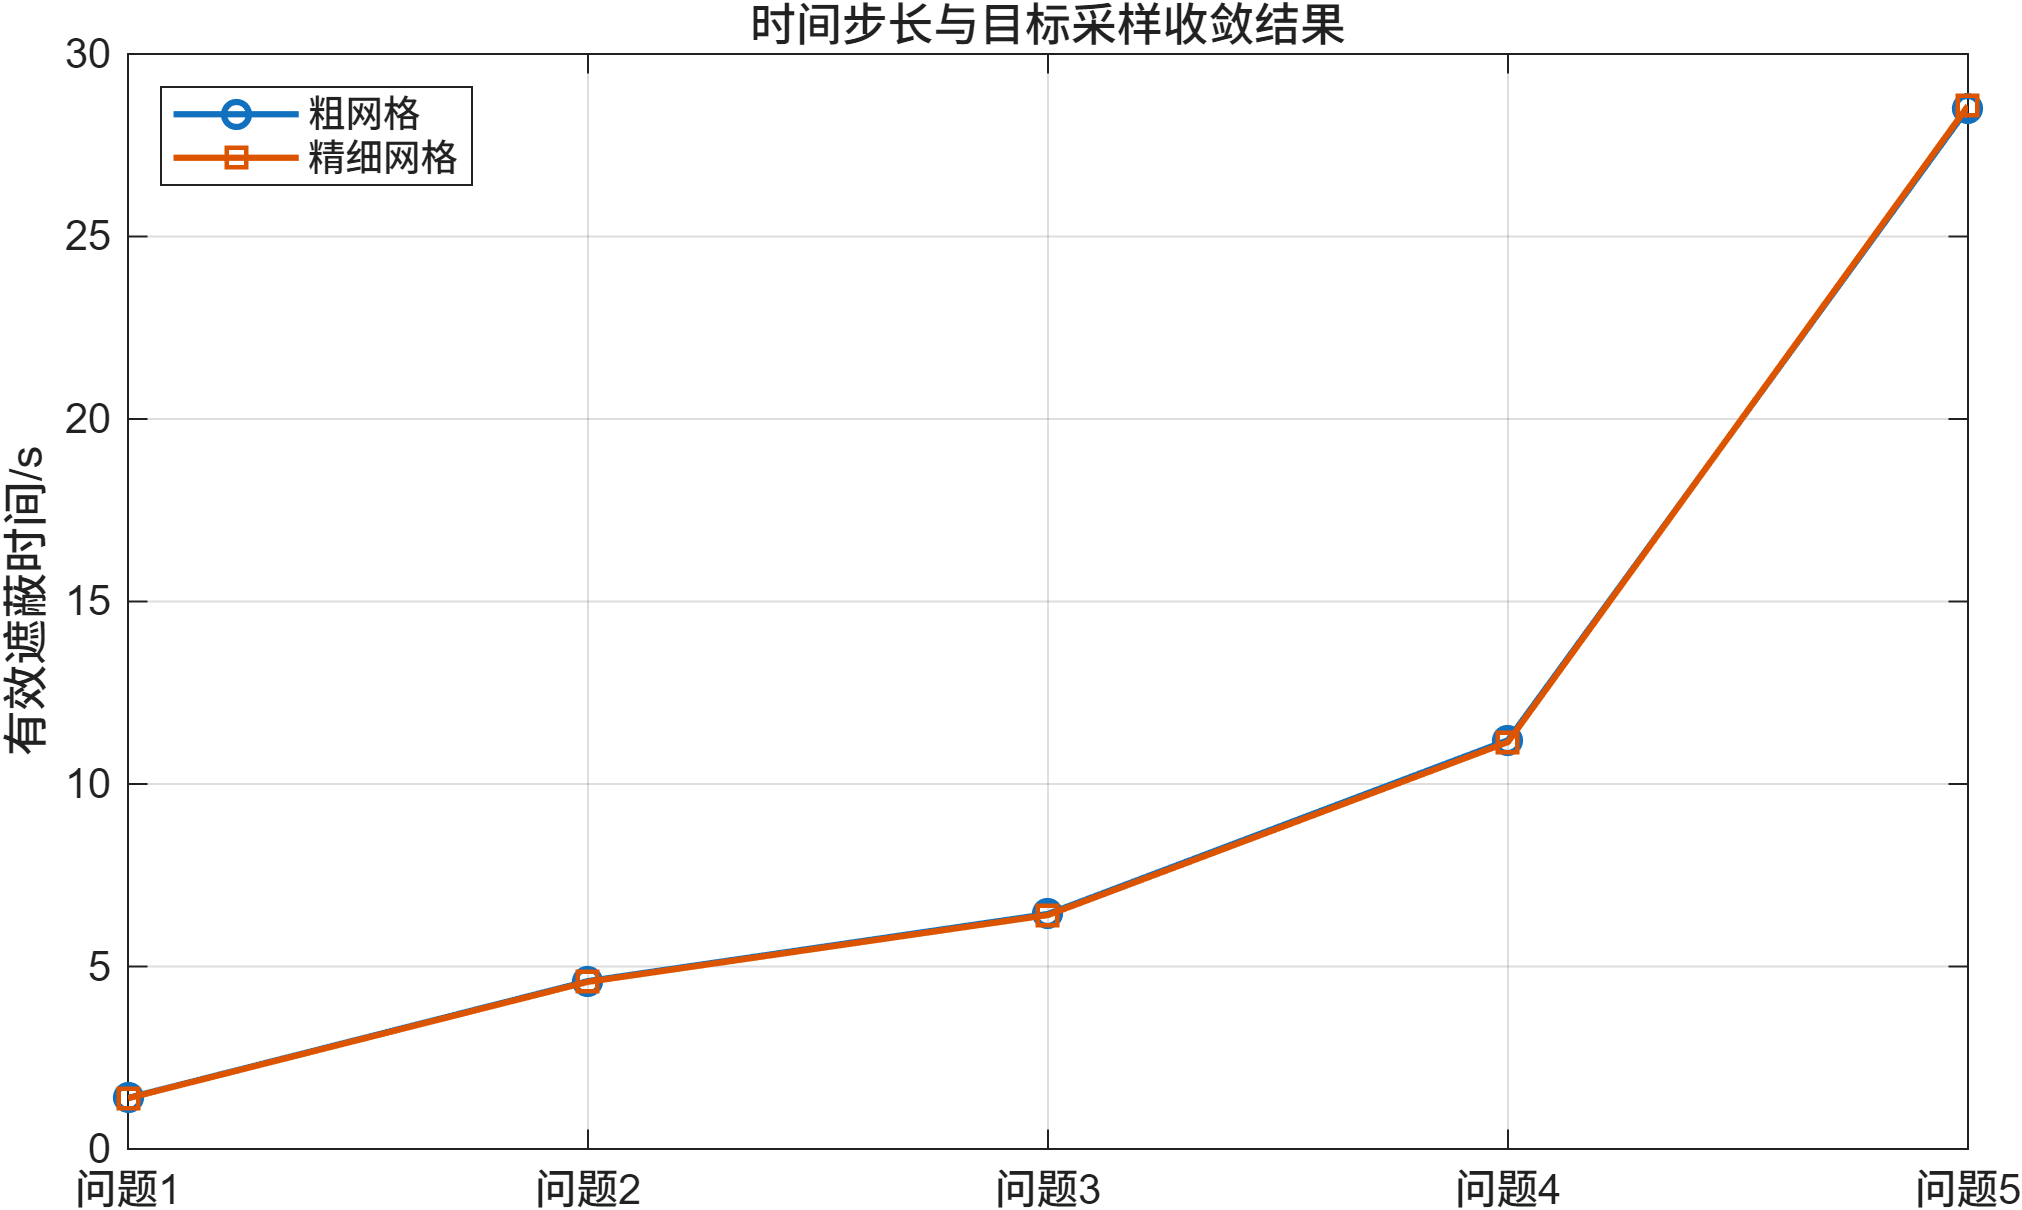
\includegraphics[width=0.72\textwidth]{figures/convergence.png}
\caption{粗、精网格下的遮蔽时间比较}
\label{fig:conv}
\end{figure}

问题5高密度结果为 $(9.960,12.490,6.130)$ s，总时长仍为28.580 s。各问随网格加密趋于稳定，正式结果保留三位小数具有合理精度。

\subsection{边际贡献检验}

对正式方案中的每枚烟幕弹计算
\begin{equation}
\Delta T_{ij}=T_j(S)-T_j(S\setminus\{i\}).
\end{equation}
问题5保留的9枚弹在高密度模型下均存在正边际贡献，说明最终后向删除已排除可在数值容差内无损移除的冗余弹。独立遮蔽时间用于填写结果表，边际贡献仅用于判断冗余和确定主要干扰目标，避免混淆两类指标。

\section{模型评价与改进方向}

\subsection{模型优点}

\begin{enumerate}[label=\arabic*)]
\item 运动学关系显式，投放点、起爆点和云团轨迹均可直接复核；
\item 完整圆柱目标判据利用了题目给出的尺寸信息，并允许多云团覆盖不同可见区域；
\item 连续代理与严格验收分离，兼顾搜索效率和结果含义；
\item 问题5采用分层优化，能够利用遮蔽空缺增量配置剩余投弹资源；
\item 通过高密度复算、边际贡献和整数规划形成多层验证链。
\end{enumerate}

\subsection{模型不足}

\begin{enumerate}[label=\arabic*)]
\item 未考虑风场、空气阻力和烟幕扩散，实际云团可能产生水平漂移和形变；
\item 严格遮蔽仍依赖时间与空间离散，区间端点存在有限网格误差；
\item 差分进化和分块局部搜索不能证明原连续模型全局最优；
\item MILP仅在有限候选库中给出零间隙证明，候选库之外仍可能存在更优航线；
\item 问题3第三枚弹未产生边际增益，仍可通过更强的事件驱动搜索继续考察。
\end{enumerate}

\subsection{改进方向}

可进一步引入风速随机扰动和鲁棒优化，以最坏情形或期望遮蔽时间为目标；采用二分法精确定位遮蔽区间端点，降低固定时间步长误差；扩充不同随机种子、跨目标投弹序列和事件驱动航线候选，再用整数规划认证更大候选库；若计算资源允许，可构造区间放松上界，给出连续全局最优值的误差区间。

\section{结论}

本文建立了烟幕干扰弹投放问题的统一运动学和完整目标几何遮蔽模型，并针对五个问题设计由解析计算、差分进化、联合局部优化、增量投弹、冗余删除及0--1整数规划组成的分层求解方法。五问严格遮蔽时长依次为1.390 s、4.580 s、6.410 s、11.170 s以及问题5总计28.580 s。问题5最终使用9枚烟幕弹，三枚导弹均获得有效且可不连续的遮蔽区间。高密度复算、边际贡献和候选集整数规划结果共同说明方案满足题目约束、数值稳定，并在当前候选库和离散精度下达到全局最优组合。

\begin{thebibliography}{99}
\bibitem{de} Storn R, Price K. Differential evolution -- A simple and efficient heuristic for global optimization over continuous spaces[J]. Journal of Global Optimization, 1997, 11(4): 341--359.
\bibitem{boyd} Boyd S, Vandenberghe L. Convex Optimization[M]. Cambridge: Cambridge University Press, 2004.
\bibitem{taha} Taha H A. Operations Research: An Introduction[M]. 10th ed. Pearson, 2017.
\bibitem{geom} de Berg M, Cheong O, van Kreveld M, Overmars M. Computational Geometry: Algorithms and Applications[M]. 3rd ed. Springer, 2008.
\bibitem{matlab} MathWorks. MATLAB Optimization Toolbox User's Guide[EB/OL]. Natick: The MathWorks, Inc., 2025.
\end{thebibliography}

\appendix
\section{主要算法伪代码}

\subsection{完整目标遮蔽判定}

\begin{lstlisting}
for each missile j
    for each time t
        find active smoke clouds
        find visible points on the cylinder
        for each visible point q
            covered(q) = any(distance(cloud, segment(Mj,q)) <= 10)
        end
        H(t) = all(covered)
    end
    T(j) = trapz(t,H)
end
\end{lstlisting}

\subsection{问题5增量优化流程}

\begin{lstlisting}
plan = initial_candidate_plan;
plan = block_refine(plan);
plan = remove_redundant_bombs(plan);

while bomb_count < 15
    candidate = search_new_bomb(plan);
    candidate = block_refine(candidate);
    if total_gain > 0.01 || ...
       (total_gain >= -0.02 && min_gain > 0.01)
        plan = candidate;
    else
        break
    end
end

plan = remove_redundant_bombs(plan);
\end{lstlisting}

\subsection{候选集整数规划}

\begin{lstlisting}
for each UAV plan p
    precompute point_cover(p, missile, time, target_point)
end

% x: selected UAV plans, y: fully covered missile-time nodes
maximize sum(dt .* y)
subject to
    y(j,n) <= sum(point_cover(p,j,n,q) * x(p)), for all q
    sum(x(plans_of_uav_k)) <= 1
    x, y are binary
\end{lstlisting}

\section{支撑文件说明}

\begin{table}[H]
\centering
\begin{tabularx}{0.95\textwidth}{lX}
\toprule
文件 & 功能\\
\midrule
\texttt{run\_all.m} & 顺序运行五问并导出三个结果表\\
\texttt{coverage\_time.m} & 完整目标严格遮蔽时间及0--1轨迹\\
\texttt{coverage\_score.m} & 连续接近度代理目标\\
\texttt{solve\_problem1.m--solve\_problem5.m} & 五个问题的求解程序\\
\texttt{add\_bombs.m} & 空缺导向的新增烟幕弹搜索\\
\texttt{validate\_results.m} & 约束、高密度时长和边际贡献验证\\
\texttt{convergence\_check.m} & 时间和空间离散收敛检验\\
\texttt{solve\_problem5\_milp.m} & 候选集0--1整数规划认证\\
\texttt{result1.xlsx--result3.xlsx} & 按题目模板填写的最终投放策略\\
\bottomrule
\end{tabularx}
\end{table}

\end{document}
